%
% hps_thesis.tex
% author: Omar Moreno 
% date: August 31, 2015
%

% Set the document type and the font size
\documentclass[12pt]{report}

% ?
\usepackage[utf8]{inputenc}

% Package required to load images
\usepackage{graphicx}

% Package used to set the layout of the page
\usepackage[left=1.5in, right=1.25in, top=1.25in, bottom=1.25in]{geometry}

% Allows double spacing of document
\usepackage{setspace}

\usepackage{subcaption}

\begin{document}

\doublespacing

%%%%%%%%%%%%%%%%
% Front Matter %
%%%%%%%%%%%%%%%%

%%%%%%%%%%%%%%%%
%   Abstract   %
%%%%%%%%%%%%%%%%

\pagestyle{plain}
The Heavy Photon Search (HPS) is a new experiment at Jefferson Lab that will 
search for heavy $U(1)$ vector bosons (heavy photons, dark photons or $A'$)
in the mass range of 10 MeV/c$^{2}$ to 1 GeV/c$^{2}$ that couple weakly to
ordinary matter.  Heavy photons in this mass range are theoretically favorable
and may also mediate dark matter interactions.  The heavy photon couples to 
electric charge through kinetic mixing with the photon, in turn, inducing an 
effective gauge coupling of the $A'$ to electric charge, which is suppressed
relative to the electron charge by a factor of 
$\epsilon \sim 10^{-2} - 10^{-12}$.  Since heavy photons couple to electrons, 
they can be produced through a process analogous to bremsstrahlung radiation, 
subsequently decaying to narrow $e^{+}e^{-}$ resonances which can be observed 
above the dominant QED trident background.  For suitably small couplings, dark
photons travel detectable distances before decaying, providing a second 
signature.

HPS will utilize this production mechanism to probe heavy photons with relative 
couplings of $\epsilon^2 \sim 10^{-5} - 10^{-10}$ and search for the 
$e^{+}e^{-}$ decay of the
heavy photon via two signatures: invariant mass and displaced vertex.  Using 
Jefferson Lab’s high luminosity electron beam incident on a thin tungsten target along with a compact, large 
acceptance forward spectrometer consisting of a silicon vertex tracker and lead
tungstate electromagnetic calorimeter, HPS will access unexplored regions in the
mass-coupling phase space. 

The HPS engineering run took place in spring of 2015 using a 1.056 GeV, 50 nA 
beam.  This dissertation will present the results of a resonance search for a heavy
photon in the mass range between 20 MeV/$c^2$ to 60 MeV/$c^2$ using a portion of the unblinded
engineering run data which amounts to a luminosity of 74 nb$^{-1}$
(.4671 mC of charge).


\chapter*{Dedication}

\tableofcontents

\listoffigures

%\chapter{Introduction}
%
%\chapter{Physics Motivation}

%\section{Motivations for an $A'$ from Dark Matter}
%\section{Current Limits of Heavy Photons}

%%%%%%%%%%%%%%%%%%%%%%%%%%%%%%%%%
%  HPS Signal and Backgrounds   %
%%%%%%%%%%%%%%%%%%%%%%%%%%%%%%%%%

\chapter{HPS Signal and Backgrounds}

The Heavy Photon Search is a fixed target experiment that will search for heavy
photons in the mass range of 20 MeV/c$^{2}$ to 500 MeV/c$^{2}$ and couplings
of $\epsilon \sim 10^{-5} - 10^{-10}$.  Since heavy photons couple to electric
charge, they can be produced by a process analogous to bremsstrahlung 
radiation.  The heavy photon subsequently decays to narrow $e^+e^-$ resonances, 
which can be observed above the dominat quantum electrodynamic (QED) trident
background.  For suitably small couplings, heavy photons travel detectable 
distances before decaying providing a second signature.  In the chapter that
follows, both the heavy photon production mechanism and background involved 
in such a search will be discussed.

\section{Heavy Photon Production}

Sensitivity to the theoretically favored regions of the heavy photon 
mass-coupling phase space can be best achieved using high luminosity fixed
target experiments \cite{PhysRevD.80.075018}.  In such experiments, an electron
of energy $E_{0}$ incident on a high $Z$ target will radiate heavy photons 
through a process analogous to ordinary photon bremsstrahlung.  The differential
(Fig. \ref{fig:ap_production}).  
\begin{figure}[t]
    \centering
    \caption{A' being produced.}
    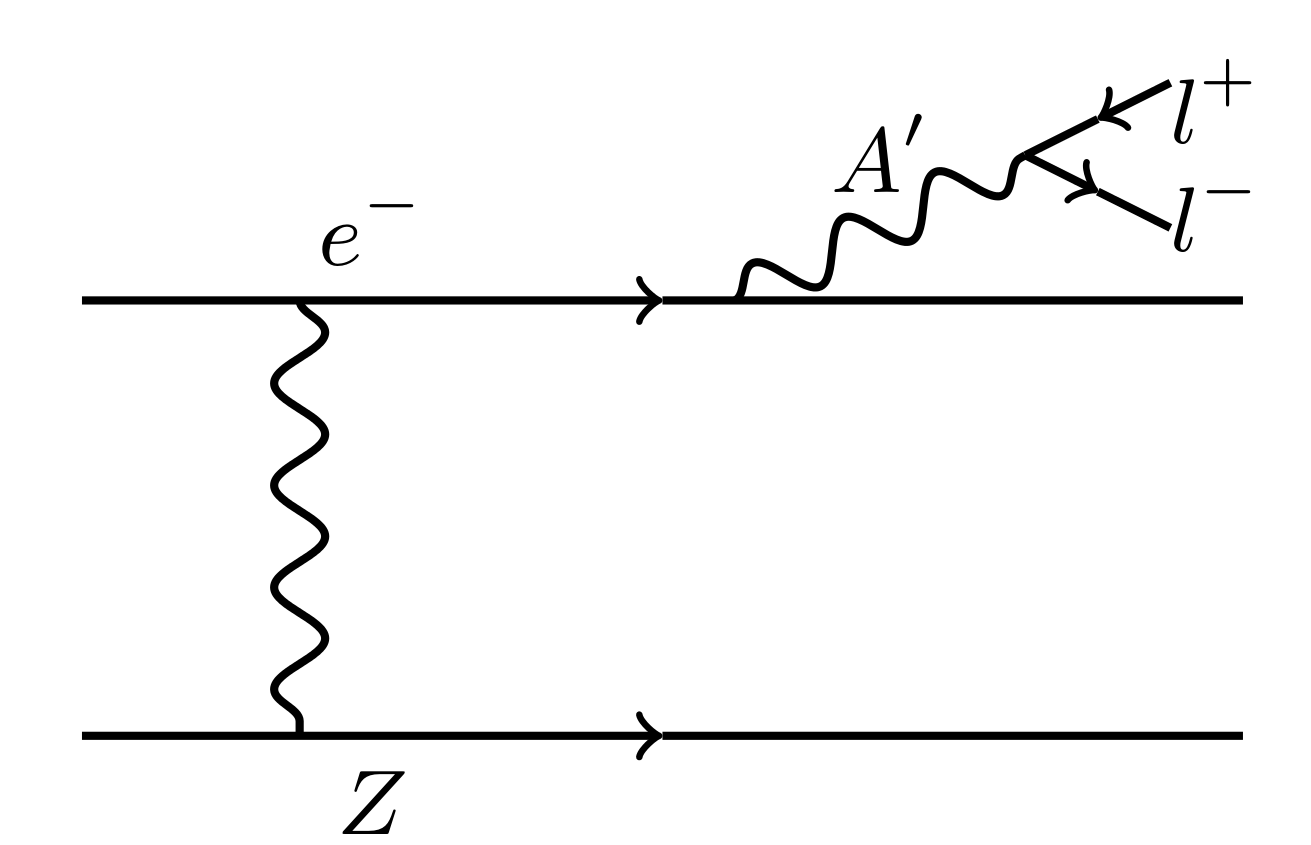
\includegraphics[width=0.5\textwidth]{images/aprime_brem.png}
    \label{fig:ap_production}
\end{figure}  
cross-section of such a process can be estimated using the Weizacker-Williams 
approximation as 
\[
    \frac{\sigma}{dx d\cos{\theta_{A}}} \approx \frac{8 Z^{2} \alpha^{3} \epsilon^{2} E_{0}x}{U^{2}} \chi
            \time [(1 - x + x^{2}/2) - x(1-x)m_{A'}^{2}E_{0}^{2}x\theta_{A'}^{2}/U^{2}]
\]
where $\alpha \sim 1/137$ is the fine structure constant, $\theta_{A}$ is the 
scattering angle of the $A'$, $\chi$ is the effective photon flux and 
\[
    U(x, \theta_{A'}) = E_{0}^{2}x\theta_{A'}^{2} + m_{A'}^{2}\frac{1-x}{x} + m_{e}^2 x
\]
is the virtuality of the intermidiate electron.

%In the case that the mass of the heavy photon is zero, equation
Although heavy photons are produced in a process similar to ordinary bremsstrahlung, 
their production rate and kinematics differ in several ways: 
\begin{itemize}
    \item The production cross-section is suppressed by a factor of $\epsilon^{2}m_{e}^{2}/m_{A'}^{2}$.
    \item The $A'$ is produced very forward.
    \item The $A'$ will take most of the incident beam energy.
\end{itemize}

\section{Trident Backgrounds}

The primary background expected to dominate the final event sample of the Heavy
Photon Search experiment is the quantum electrodynamic Trident process.  As 
shown on Fig. (), the tridents can be seperated out into two main diagrams: 
\begin{figure}[t]
    \centering
    \caption{A' being produced.}
    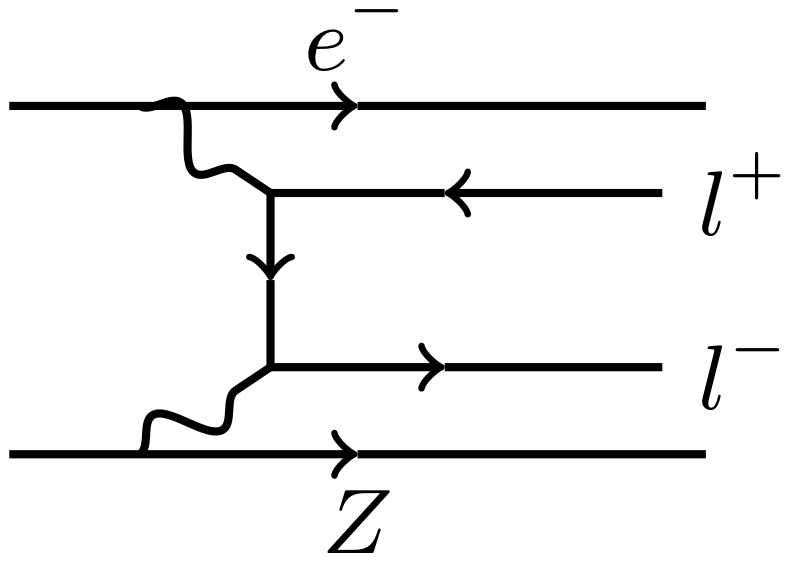
\includegraphics[width=0.5\textwidth]{images/bethe-heitler.png}
    \label{fig:tridents}
\end{figure}  
Bethe-Heitler and radiatives. The kinematics of radiativesare indistinguishable
from the $A'$ signal events within an invariant mass window near the $A'$ mass.
Therefore, radiatives can be used to analyze both the rate of the $A'$ signal 
production and the sensitivity of an experiment to $A'$ signals.  Specifically,
the $A'$ production cross-section is related to the production cross-section of 
radiatives as 
\[
    \frac{d\sigma(A')}{d\sigma(\gamma^*)} = \frac{3\pi\epsilon^{2}}{2 N_{eff} \alpha}
        \frac{m_{A'}}{\delta m}
\]
As a result, the radiatives in the final event sample can be used to analyze 
the $A'$.

Although the rate of the Bethe-Heitler process dominates among the two processes, 
its different kinematics can be used to reduce them in the final event sample.
Specifically, the $A'$ decay products are highly boosted while the recoiling 
electron is soft and scatters at large angles.  In contrast, at higher 
energies, the Bethe-Heitler process is not enhance.  Furthermore, only one of
the leptons in the pair will be highly boosted, while the other will be much
softer.  The recoiling electron will be produced much more forward.




%%%%%%%%%%%%%%%%%%%%%
%   HPS Apparatus   %
%%%%%%%%%%%%%%%%%%%%%

\chapter{The HPS Apparatus}

%The HPS experiment engineering run was conducted in the Spring of 2015 at the
%Thomas Jefferson National Accelerator Facility (JLab) in Newport News, VA.  The
%HPS detector was installed within the Hall B alcove upstream of the Continuous 
%Electron Beam Accelerator Facility (CEBAF) Large Acceptance Spectrometer for 12
%GeV (CLAS12) detector.  HPS utilized CEBAF's high luminosity electron beam,
%operating at an energy of 1.056 GeV and current of 50 nA, incident on a thin
%(~0.125\% $X_{0}$) tungsten target to search for an $A'$ with a mass in the 
%range of 20 - 100 MeV.  

At the energies at which the HPS experiment is operating, the 
electroproduced $A'$ will carry most of the incident beam energy. Consequently,
the $A'$ decay products will be highly boosted, necessitating a detector with very
forward acceptance that can be placed in close proximity to the target.
Maximizing the acceptance requires placing the detector close to the beam plane,
encroaching on a ``dead zone'' which is occupied by an intense flux of multiple
Coulomb scattered beam particles along with radiative secondaries originating
from the target.  In order to avoid additional background from from beam gas
interactions, the detector needs to operate in vacuum. Finally, minimizing the
material budget of the active area of the detector is essential to reducing the
multiple scattering that dominates both the mass and vertex resolutions that
determine the experimental sensitivity.

These design principles led to the conception of the HPS detector.  
Specifically, HPS utilizes a compact, large acceptance forward spectrometer 
consisting of a silicon microstrip tracker (SVT) along with a lead tungstate
electromagnetic calorimeter (Ecal).  The SVT is installed inside of a vacuum
chamber and inside of an analyzing magnet immediately downstream of a thin
($0.125\%X_{0}$) tungsten target.
The Ecal is placed downstream of the tracker and provides the primary 
trigger for the experiment and is also used for electron identification. Together, 
both subsystems provide the complete kinematic information required to 
reconstruct heavy photons.

The HPS detector was installed and commissioned within the Hall B alcove at the
Thomas Jefferson National Accelerator Facility (JLab) in Newport News, VA early
in the Spring of 2015. Shortly after, an engineering run took place utilizing
the Continuous Electron Beam Accelerator Facility (CEBAF) operating at an 
energy 1.056 GeV and current of 50 nA.

The chapter that follows will detail various elements of the experiment.
It will begin with a discussion of CEBAF and continue with descriptions
of several beamline elements, SVT, Ecal and data acquisition system (DAQ).

\section{CEBAF}

CEBAF's ability to provide a nearly continuous, clean and intense electron
beam makes it ideal to search for heavy photons with weak couplings. Recently,
CEBAF underwent an upgrade that increased its maximum operating energy to 12
GeV and introduced a new experimental hall, Hall D, that will house the
GlueX detector \cite{Dudek:2012vr}.  The upgraded facility is now capable of 
delivering 11 GeV electron beams to the three existing experimental halls
(Hall A, B, C) and can use the 12 GeV electron beam to generate and deliver a 9
GeV photon beam to Hall D. 

As shown on Figure \ref{fig:cebaf}, achieving 12 GeV operation, required several
improvements to the accelerator \cite{Burkert:2012rh}. Central to the upgrade 
was the addition of 5 
cryomodules to each of the linacs.  Coupled with upgrades to the accelerator
magnets and power supplies, the additional cryomodules allowed each linac to
accelerate electrons at a rate of 2.2 GeV per pass up to a maximum of 5 passes.
\begin{figure}[h]
    \centering
    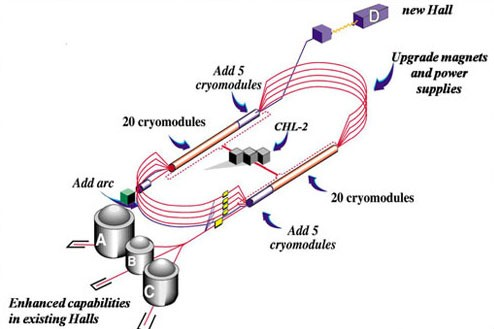
\includegraphics[width=0.9\textwidth]{images/cebaf.jpg}
    \caption{A diagram of the Thomas Jefferson National Accelerator Facility
             Continuous Electron Beam Accelerator Facility showing the 
             components that were upgraded as part of the 12 GeV Upgrade 
             program.}
    \label{fig:cebaf}
\end{figure}
Enabling four hall operation also required the addition of a new 750 MHz RF 
separator, a new laser to the electron source and a 10th arc which provides
the additional pass of acceleration that allows 
delivery of the maximum beam energy to Hall D.


\subsection{Electron Production and Injection}

%
%  Note: I need to make sure that this is still correct in the 12 GeV era.
%
The electrons injected into the accelerator were produced by photoemission from
a strained GaAs superlattice photocathode \cite{Maruyama:2004hx}.  Each of the 
four experimental halls has a dedicated gain-switched fiber coupled laser of
wavelength 1560 nm.  The lasers are frequency doubled in order to produce light
of wavelength of 780 nm, matching the band gap of the superlattice cathode. The
lasers are phased shifted and are each pulsed for $\approx$ 40 ps at the 
frequency of 499 MHz.  Since the operational frequency of the accelerator 
cryomodules is 1497 MHz, four hall operation requires subharmonics of 499 MHz to
be chosen.  This is achieved by ``cutting away'' pulses using an optical 
modulator \cite{Kazimi:2013yua}.


The photoemission electrons are released into an extremely high vacuum
environment at a pressure of $10^{-11}$ to $10^{-12}$ Torr.  The free electrons
are then delivered into the injector by a 100 keV electron gun.  The injector
itself then accelerates the electron bunches to an energy of 50 MeV 
%by 2 1/4 cryomodules 
before being delivered into the accelerator.

\subsection{Electron Acceleration}

The CEBAF accelerator is composed of two linacs arranged in a racetrack
configuration as shown on Fig \ref{fig:cebaf}. Each of the linacs consist
of 25 cryomodules, 5 of which were added as part of the upgrade.  The original
(new) cryomodules consist of 8 5-cell (7-cell) superconducting radio frequency
(RF) cavities made of ultra-pure Niobium (see Figure \ref{fig:cebaf_cavity}).  
The original cryomodules
\begin{figure}[h]
    \centering
    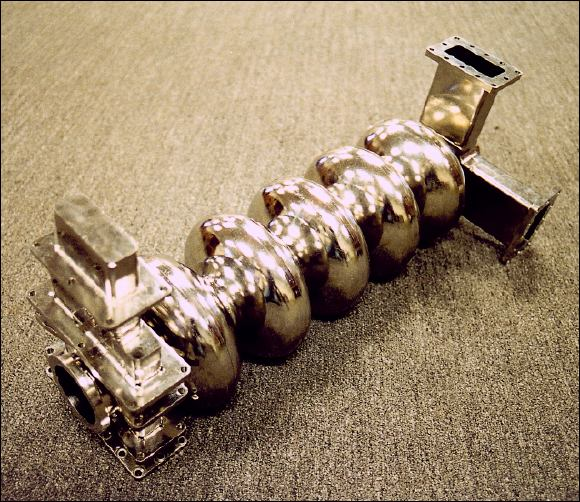
\includegraphics[width=0.7\textwidth]{images/cebaf_cavity.jpg}
    \caption{A 5-cell ultra-pure Niobium superconducting radio frequency cavity
             used to accelerate electrons at CEBAF.}
    \label{fig:cebaf_cavity}
\end{figure}
are capable of accelerating an electron upwards of 25 MeV while the newly installed
cryomodules can achieve an acceleration of 100 MeV.  This leads to an acceleration
of 1.1 GeV per linac and 2.2 GeV per pass. The 
number of passes depends on the energy requirements of the experiment taking place.
However, for electrons delivered to Halls A, B and C, the maximum amount of passes
is 5 while for Hall D, it's 5.5.

Electron bunches circulating the accelerator can be delivered to a Halls A, B
and C by an RF separator operating at a frequency of 499 MHz.  Delivery to Hall
D uses an RF separator of 750 MHz.

\subsection{Single Pass Operation For HPS}

During the Spring of 2015, HPS was prepared to run at a beam energy of 2.2 GeV,
in conjuction with the commissioning of the 750 MHz RF separator.
Unfortunately, an incident occurred which resulted in the loss of the new CHL
required to operate the accelerator as a 12 GeV machine.
The loss caused the accelerator to 
fallback to 6 GeV operation using a single CHL.  As a result, HPS was given
the unique opportunity to run with a beam energy of 1.056 GeV allowing the
experiment to have sensitivity to the g-2 favored region of the mass-coupling
phase space.  

\section{Beamline}

\subsection{Layout}

The HPS experiment is installed within the Hall B alcove and utilizes a 
three-magnet chicane system as shown on Figure \ref{fig:beamline}. 

\subsection{Beam Quality}

In order to optimize the ve





%The first and last dipoles of the chicane,  are used to bend
%the beam into the HPS apparatus while the second dipole, the Hall B pair 
%spectrometer, serves as the analyzing magnet of the experiment.  

\begin{sidewaysfigure}
    \centering
    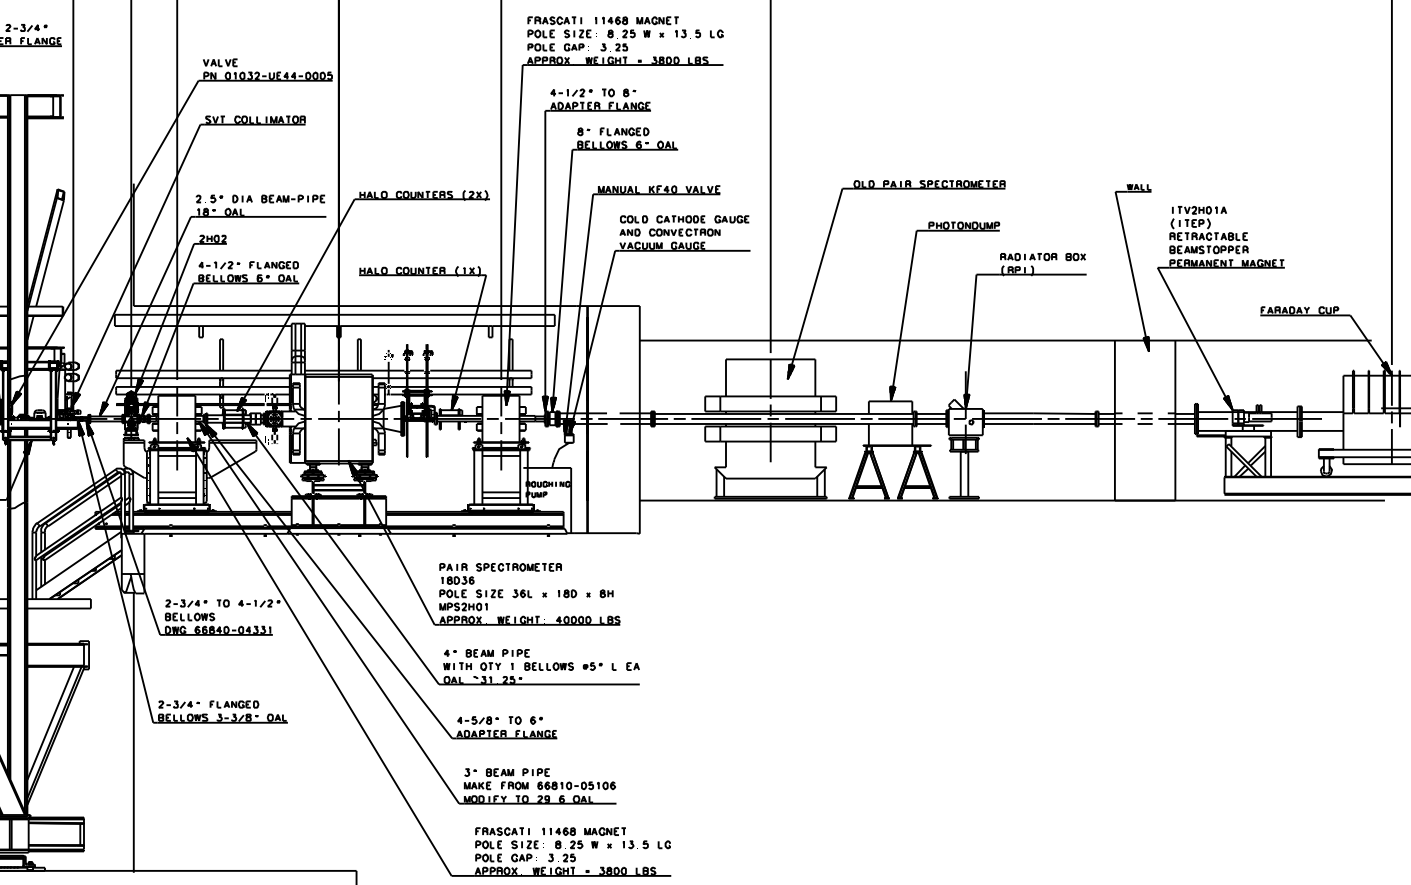
\includegraphics[width=\textwidth]{images/beamline.png}
    \caption{Configuration of the beam line during the HPS engineering run.}
    \label{fig:beamline}
\end{sidewaysfigure}

\section{Silicon Vertex Tracker}

\subsection{Layout}

The HPS SVT is comprised of two halves of six measurement layers encroaching the
beam plane as shown of Figure \ref{fig:svt_layout_render}. Each layer consist of a pair of
closely-spaced silicon planes with one of the planes oriented orthogonal to
the beam plane and the other at small angle stereo 
(see Table \ref{tab:svt_layout}).
\begin{figure}[h!t]
    \centering
    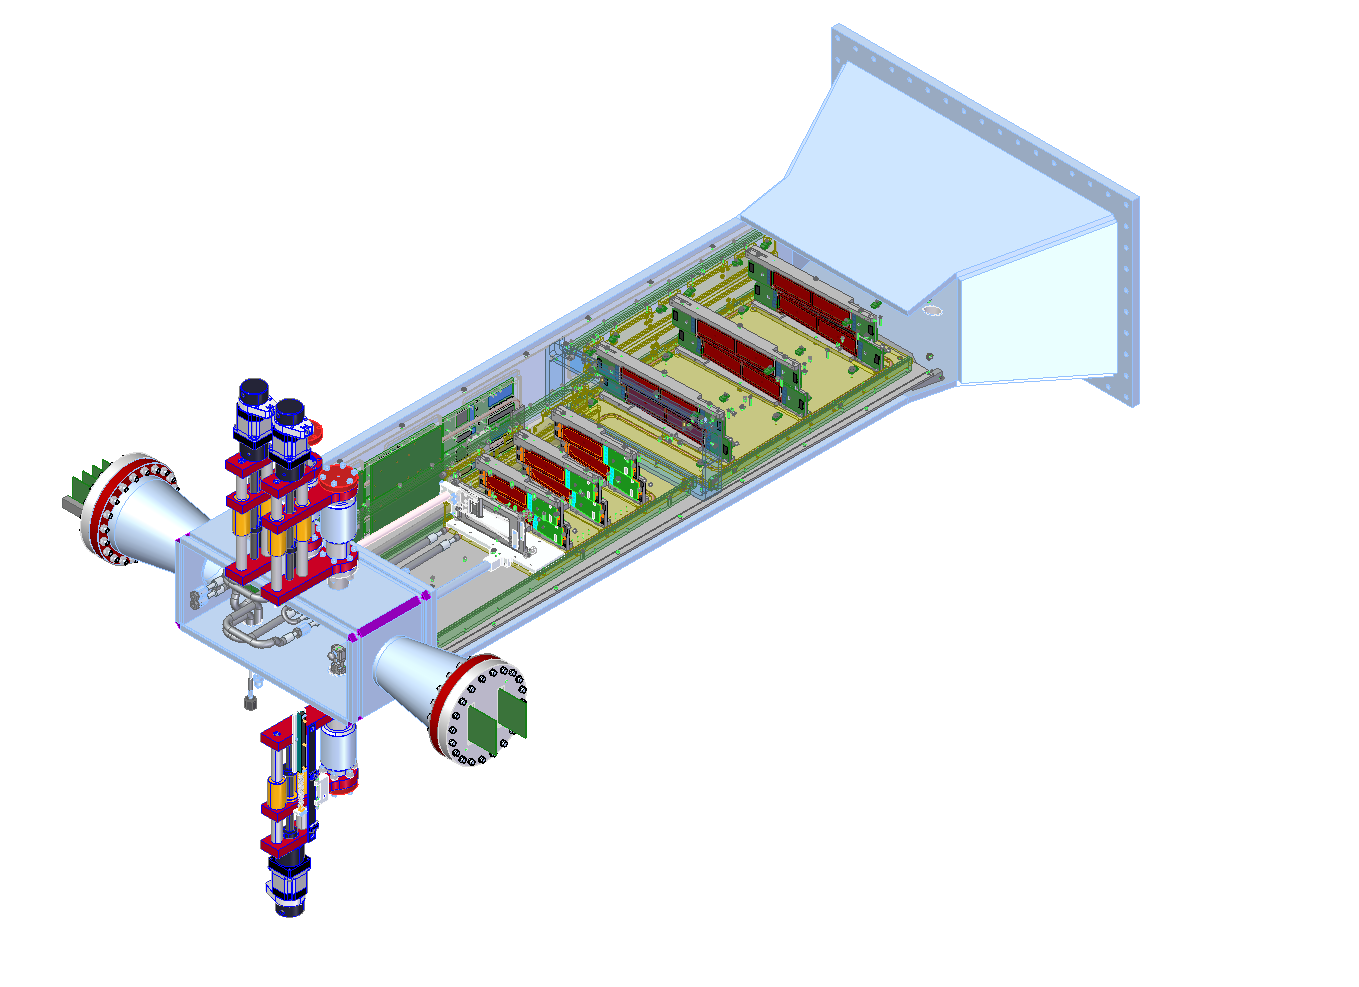
\includegraphics[width=0.9\textwidth]{images/svt_layout_render.png}
    \caption{A rendered view of the Silicon Vertex Tracker inside of the pair
             spectrometer vacuum chamber.}
    \label{fig:svt_layout_render}
\end{figure}
This allows
for the measurement of both the vertical and horizontal coordinate of a hit, in turn, 
enabling full 3D hit reconstruction.  

The first three layers consist of a single sensor of coverage above and below
the beam plane and use a stereo angle of 100 mrad. In order to better match the
% needs a sentence explaining why 100 mrad stereo was used.  According to the
% proposal, it balances acceptance against vertexing resolution.
acceptance of the Ecal, the coverage of the last three layers is two sensors 
wide and use a stereo angle of 50 mrad.  The choice of a 50 mrad angle for the
last three layers instead of 100 mrad was meant to break the degeneracy that
results in fake tracks
due to ghost hits in layers with the same stereo angle.  It must be noted that
only five layers are needed to match the full acceptance of the Ecal, however,
an improvement in the momentum resolution was observed with the addition of 
another layer.  In total, the SVT makes use of 36 sensors, which amounts to 
23,004 channels.

Since heavy photons are produced very forward, and the opening angle of their 
decay products goes as $\sim m_{A}/E_{0}$, sensitivity to low mass heavy photons
requires
the tracker layers to be as close to the beam plane as possible.  When deciding
the distance of the first layer to the beam, several effects needed to be taken
into consideration. These include the extent of the beam halo, the amount of 
radiation damage that is expected to be incurred from the Coulomb scattering
of the primary beam as well as radiative secondaries, the ability to resolve 
hits with pileup present and being capable of doing pattern recognition in a high 
occupancy environment.  With all of this in mind, it was determined that the 
closest tolerable distance was 15 mrad, putting the active edge of layer 1 
at 0.5 mm from the beam center. In simulation, this corresponds to 1\% occupancy
of strips closest to the beam plane of layer 1.

% I should talk about the positions as surveyed.
%The SVT layout is summarized in Table \ref{tab:svt_layout}. \textbf{Talk about
%the survey}.

%%%%%%%%%%%%%%%%%%%%%%%%%%%
%%% Table of SVT layout %%%
%%%%%%%%%%%%%%%%%%%%%%%%%%%
% I should use the survey positions here.
%\begin{table}[t]
\begin{sidewaystable}
    \centering
    \begin{tabular}{lcccccc}  
        \toprule
        \textbf{Layer} & \textbf{1} & \textbf{2} & \textbf{3} & \textbf{4} & \textbf{5} & \textbf{6} \\
        \midrule
        \midrule
        $z$ position from target (cm)    & 10 & 20 & 30 & 50 & 70 & 90 \\
        Stereo angle (mrad) & 100 & 100 & 100 & 50 & 50 & 50 \\
        Bend plane resolution ($\mu$m) & $\approx$6 & $\approx$6 & $\approx$6 & $\approx$6 & $\approx$6 & $\approx$6 \\
        Non-bend plane resolution ($\mu$m) & $\approx60$ & $\approx60$ & $\approx60$ & $\approx120$ & $\approx120$ & $\approx120$ \\
        Nominal dead zone in $y$ (mm) & $\pm$ 1.5 & $\pm$ 3.0 & $\pm$ 4.5 & $\pm$ 7.5 & $\pm$ 10.5 & $\pm$ 13.5 \\ 
        Material budget & .7\% & .7\% & .7\% & .7\% & .7\% & .7\% \\
        \bottomrule
    \end{tabular}
    \caption{The layout of the HPS SVT.}
    \label{tab:svt_layout}
\end{sidewaystable}
%%%%%%%%%%%%%%%%%%%%%%%%%%%

\subsection{Sensors}

At the energies at which HPS operates, the uncertainty in both the mass and
vertex resolutions are dominated by multiple Coulomb scattering in the first 
few layers.  This made it important to choose a sensor technology that would 
minimize the material budget of the SVT modules, especially since the material
budget of the sensors dominates the total material budget of the SVT modules.
Furthermore, the need to place the SVT in close proximity
to the beam plane made it necessary to choose sensors which are highly tolerant
to radiation.  With these 
considerations in mind, a readily available batch of silicon microstrip sensors,
initially manufactured for the D0 Run IIb upgrade, were found to satisfy all 
necessary requirements \cite{D0Collab:2003}.

The sensors were manufactured by Hamamatsu Photonics Corporation on 
$\langle 100 \rangle$ crystal rotation silicon and are $p^{+}$ on $n$-bulk, 
single sided, AC-coupled and polysilicon-biased. The cut dimensions of the 
sensors are $100 \times 40.34$ mm$^{2}$ with an active area of 
$98.33 \times 38.34$ mm$^{2}$. They are $320 \pm 20 \mu$m thick and have a sense
(readout) pitch of 30 (60) $\mu$m. The sensor specifications are summarized on 
Table \ref{tab:sensor_specs}.
\begin{table}[t]
    \centering
    \begin{tabular}{lr}
        \toprule
        Cut dimensions (L$\times$W)     & 100 mm x 40.34 mm \\
        Active area (L$\times$W)        & 98.33 mm x 38.34 mm \\
        Readout (Sense) pitch           & 60 (30) $\mu$m \\
        \# Readout (Sense) strips       & 639 (1277) \\
        Breakdown voltage               & $>1000$ V \\
        Depletion voltage               & $> 130$ V \\
        Bias Resistor Value             & $0.8 \pm 0.3$ M$\Omega$ \\
        AC Coupling Capacitance         & $>12$ pF/cm \\
        Total Interstrip Capacitance    & $< 1.2$ pF/cm \\
        Defective Channels              & $<1$ \% \\
        \bottomrule
    \end{tabular}
    \caption{Specifications of the sensors used for the HPS SVT.}
    \label{tab:sensor_specs}
\end{table}

Over the lifetime of the HPS detector, the sensor strips closest to the beam 
plane are expected to see $>10^{15}$ electrons per cm$^2$.  The radiation
damage the sensors are expected to incur due to the large electron flux,
will lead to an increase in both the leakage current and the voltage required to 
fully deplete the sensor.  It was then beneficial to choose a sensor technology
that can be operated at high bias voltage in order for them to remain fully
depleted even after irradiation. In fact, previous studies have shown that 
sensors that may be operated to 1000 V can tolerate a dose of 
$1.5 \times 10^{14}$ 1 MeV neq/cm$^2$ \cite{Fretwurst:2002vb}.  Since the damage
incurred by electrons with energies less than 10 GeV is a factor $\sim$ 30 less
than 1 MeV neutrons \cite{Rashevskaya:2002nd},
then ensuring all sensors can be biased to 1000 V will ensure that the sensors
will be able to withstand the expected flux of electrons over the lifetime of
HPS. 


Before being considered for use for the SVT modules, all sensors were electrically 
characterized.  Specifically, the leakage current was measured as a function
of bias voltage up to a maximum bias of 1000 V.  During these test, leakage 
currents of less than 500 nA were observed.  The measured IV curves for a subset
of sensors can be seen on Fig. \ref{fig:sensor_iv_curves}.  Only sensors whose
leakage current did not uncontrollably increase (i.e. breakdown) before reaching
a bias of 1000 V  were considered for use in HPS.
\begin{figure}[t!]
    \centering
    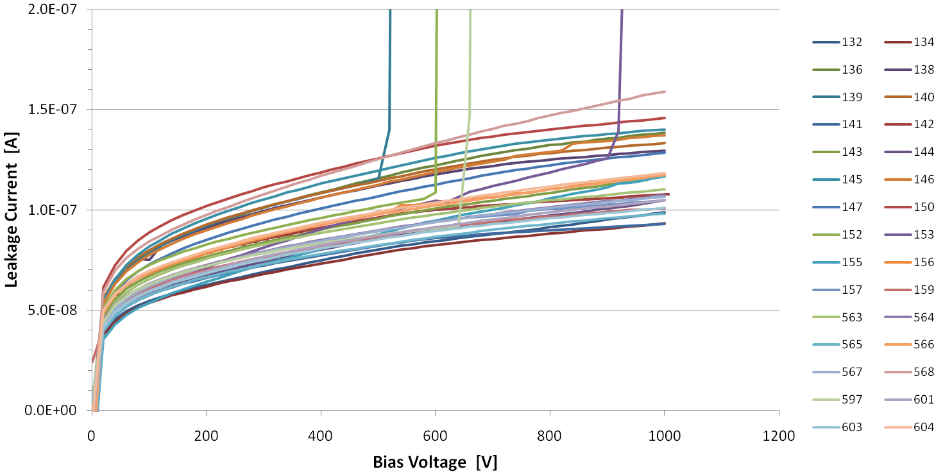
\includegraphics[width=\textwidth]{images/sensor_iv_curves.png}
    \caption{Measured IV curves for a subset of sensors used by HPS.}
    \label{fig:sensor_iv_curves}
\end{figure}

\subsection{Readout} \label{subsec:readout}

The sensors are continuously read out using the APV25 readout chip developed for
the Compact Muon Solenoid detector at the Large Hadron Collider 
\cite{Raymond:2000ey}. The APV25 has 128 channels, with each channel consisting
of a charge sensitive pre-amplifier coupled to CR-RC shaping amplifier and a 192
cell deep analog pipeline.  A schematic of a single channel is shown on 
Fig. \ref{fig:apv25_schem}.
\begin{figure}
    \centering
    \includegraphics[width=\textwidth]{images/apv25_channel_schematic.png}
    \caption{A schematic of a single channel of the APV25 readout chip.}
    \label{fig:apv25_schem}
\end{figure}

When a particle traverses a sensor, it generates a charge signal which is 
processed by the APV25 amplifier chain.  As shown on Figure 
\ref{fig:apv25_pipeline}, the shaper
\begin{figure}
    \centering
    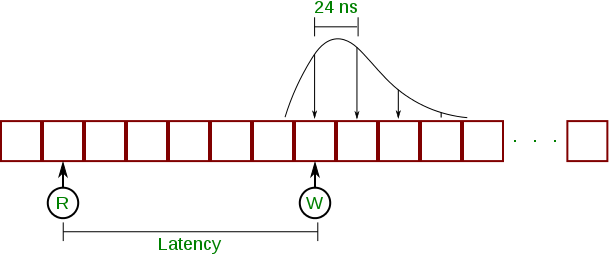
\includegraphics[width=\textwidth]{images/apv25_pipeline.png}
    \caption{A schematic demonstrating the sampling of the shaper signal and
             the management of read/write pointers.}
    \label{fig:apv25_pipeline}
\end{figure}
output is continuously sampled at 41.6 MHz into the analog pipeline. The position
along the pipeline into which the shaper output is stored is determined by 
a write pointer which continuously cycles the pipeline.  Similarly, a read 
pointer determines the position that will be marked for read out when a trigger
signal is received.  Since the trigger decision cannot happen instantaneously,
the distance between the read and write pointers or latency is programmable.
Given that only 160 pipeline cells out of the 192 are used
to buffer samples, the delay between a signal and the arrival of the trigger can
be as long as 3.8 $\mu s$. The remaining 32 cells along the pipeline are used 
to buffer the addresses of samples that are waiting to be read out.

The samples  are readout out by the Analog Pulse Shape Processor (APSP) which
can operate in two modes: peak and deconvolution mode.  In peak
mode, only a single pipeline cell is read out corresponding to the maximum 
value of the shaper output.  In deconvolution mode, three consecutive samples are
read out allowing for the reconstruction of the shaper output.  The output of 
the APSP is then sent to a 128:1 multiplexer which then makes the raw data 
frames. 
%An example of the output data frame is shown on Figure \ref{}.

During the engineering run, the APV25s were operated using the nominal settings
with listed on Table \ref{tab:apv_specs}.  At nominal, the shaping time is set
to 50 ns.  The high occupancies expected during the engineering
run meant that overlapping of hits or ``pile-up'' were a concern.  In order to 
mitigate this problem, the APV25's were operated in deconvolution allowing 
the reconstruction of the shaper output.  Furthermore, 
with each Ecal trigger, the APV25's were sent two consecutive trigger signals 
allowing the readout of six consecutive samples instead of three.  The trigger
latency was then adjusted such that two samples before the signal were readout, 
allowing the shape of the pileup pulse to be captured by the fit.  This was 
used to remove any effects of pileup from the signal pulse.  Approximately 5\%
of hits in layer were observed to be affected by pileup.
\begin{table}[ht]
    \centering
    \begin{tabular}{llr}
        \toprule
        \textbf{Name} & \textbf{Description} & \textbf{Value} \\
        \midrule
        \midrule
        IPRE   & Preamp input FET current       & 98 (460 $\mu$A)\\
        IPCASC & Preamp cascode current         & 52 (60 $\mu$A) \\
        IPSF   & Preamp source follower current & 34 (50 $\mu$A) \\
        ISHA   & Shaper input FET current bias  & 34 (50 $\mu$A) \\
        ISSF   & Shaper source follower current & 34 (50 $\mu$A) \\
        IPSP   & APSP current                   & 55 (80 $\mu$A) \\
        IMUXIN & Multiplexer input current      & 34 (50 $\mu$A) \\
        VFP    & Preamp feedback voltage        & 30  \\
        VFS    & Shaper feedback voltage        & 60  \\
        VPSP   & APSP Voltage level             & 40  \\
        LATENCY & Trigger latency               & 147 \\
        MUXGAIN & Multiplexer gain              & 100 $\mu$A/MIP \\
        \bottomrule
    \end{tabular}
    \caption{APV25 specs used during the engineering run.}
    \label{tab:apv_specs}
\end{table}
%\ref{fig:apv_shape}.
%\begin{figure}
%    \centering
%    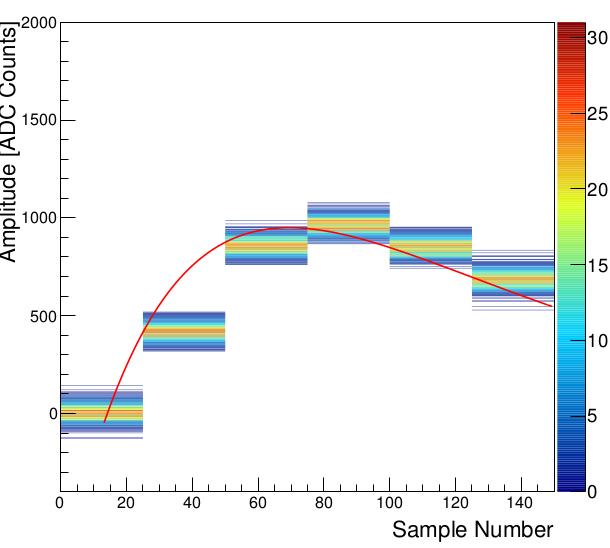
\includegraphics[width=0.9\textwidth]{images/sideB_response_ch535.png}
%    \caption{The signal shape observed during the engineering run.}
%    \label{fig:apv_shape}
%\end{figure}

\subsection{SVT Modules}

Each of the layers of the SVT consist of a ``module'' built by placing
two ``half-modules'' back-to-back around an aluminum cooling block.  The 
half-modules used for layers 1-3 are composed of a single sensor
and FR4 hybrid electronic board glued onto a polyimide-laminated carbon fiber
composite backing.  In order to better match the acceptance of the Ecal, 
the half-modules used in layers 4-6 consist of two sensors glued end-to-end onto
the polyimide-laminated carbon fiber backing with hybrids on either side of them.


%Due to space constraints, the hybrids used
%by layers 4-6 have smaller footprint.  In order to further minimize the 
%amount of material, a window is machined in the carbon fiber leaving the middle
%of the sensor exposed. Fig. \ref{fig:l13_hm} and \ref{fig:l46_hm} show both a layer 1-3 and 4-6 
%half-modules.


%Reading out of a sensor requires the use of 5 APV25 chips.


%An SVT ``half-module'' consist of an electronic readout board, 



%Each sensor requires 5 APV25 chips in order to readout all channels.  The 5 
%APV25 chips are mounted on a FR4 electronic readout board, or hybrid, containing
%filtering for the high voltage bias and a temperature sensor.  Since the pitch
%of the APV25 and the sensors are similar, the chips were wirebonded directly to
%the sensors without the need of a pitch adapter.

\begin{figure}
    \centering
    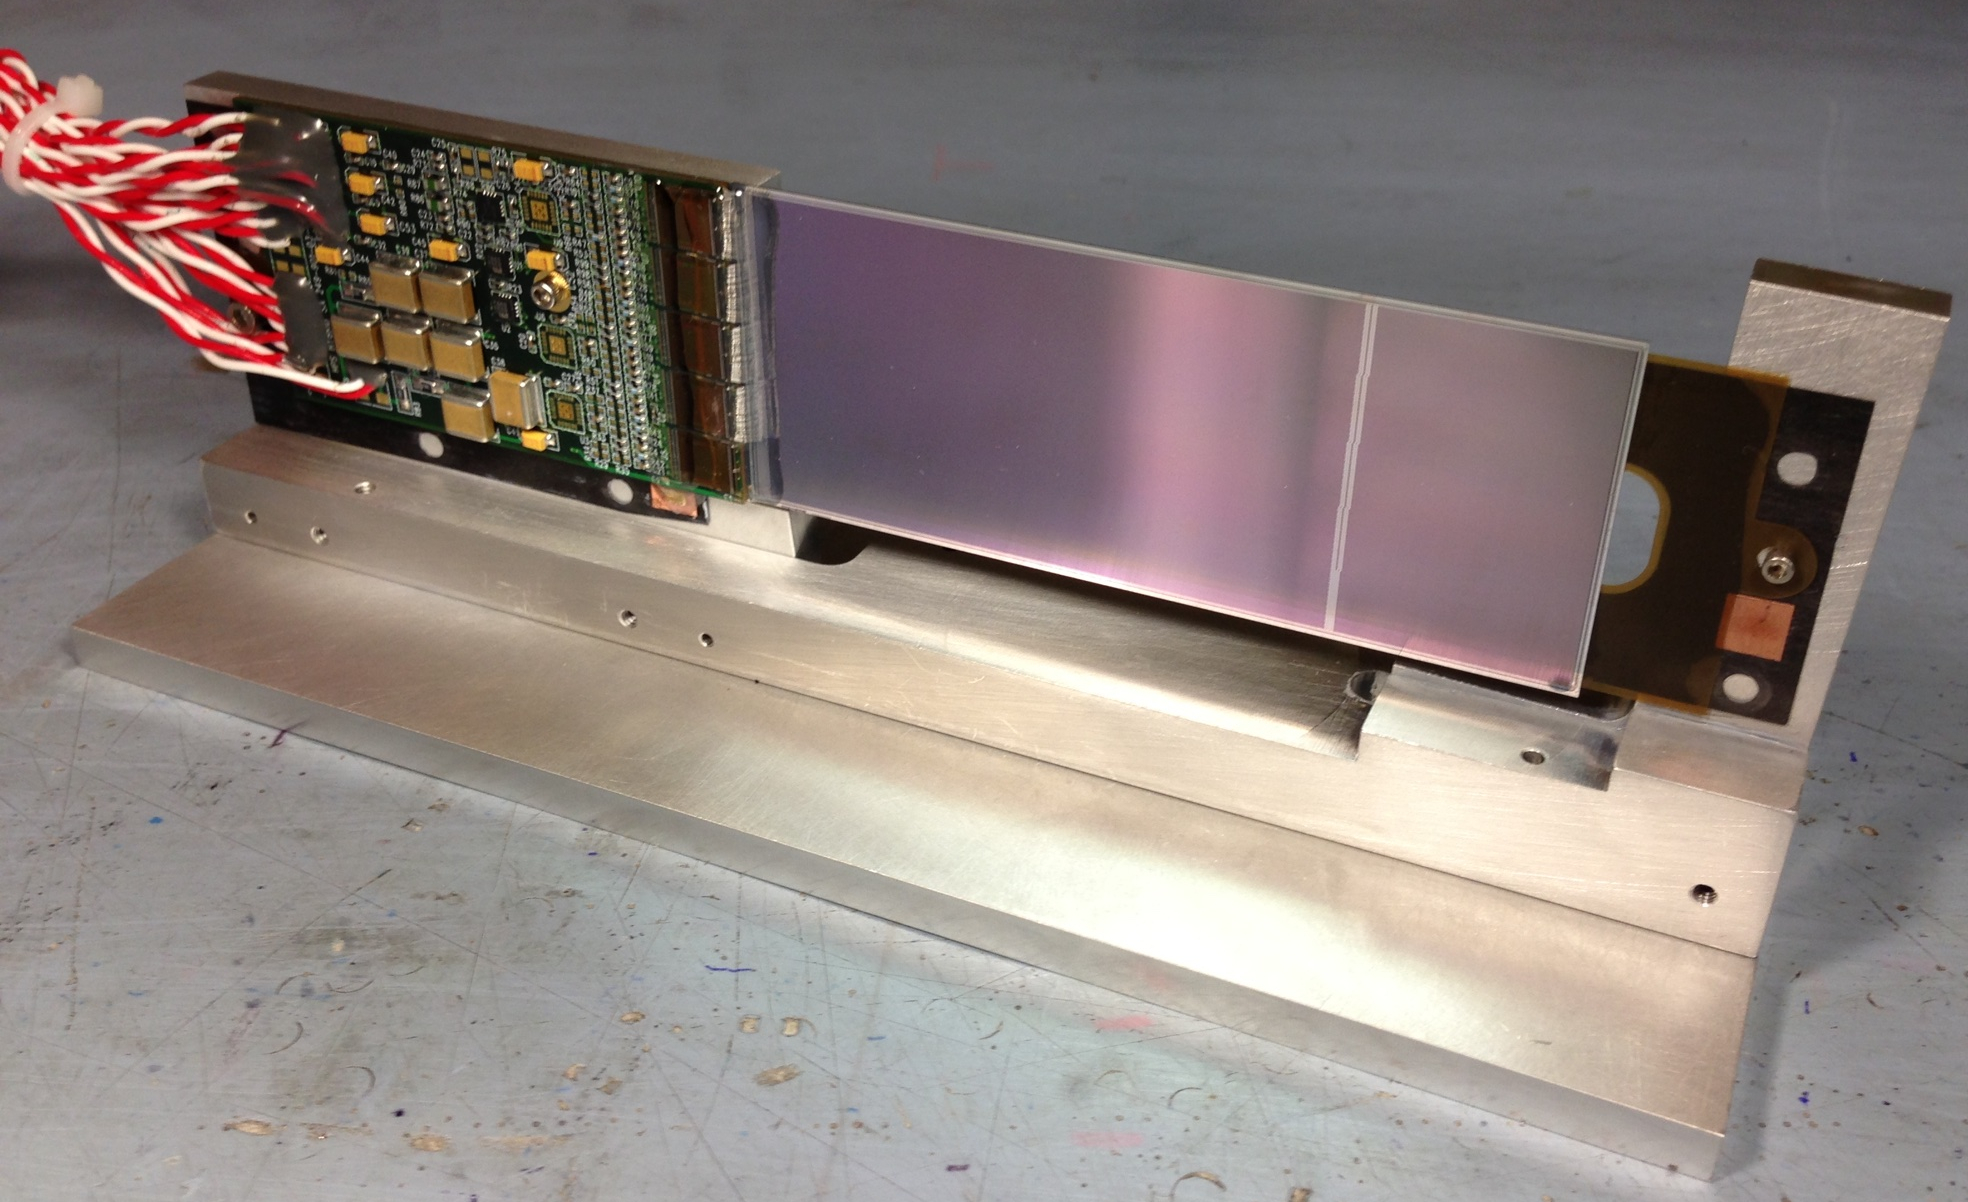
\includegraphics[width=0.9\textwidth]{images/l13_half_module.jpg}
    \caption{A layer 1-3 half-module used by the SVT. }
    \label{fig:l13_hm}
\end{figure}
\begin{figure}
    \centering
    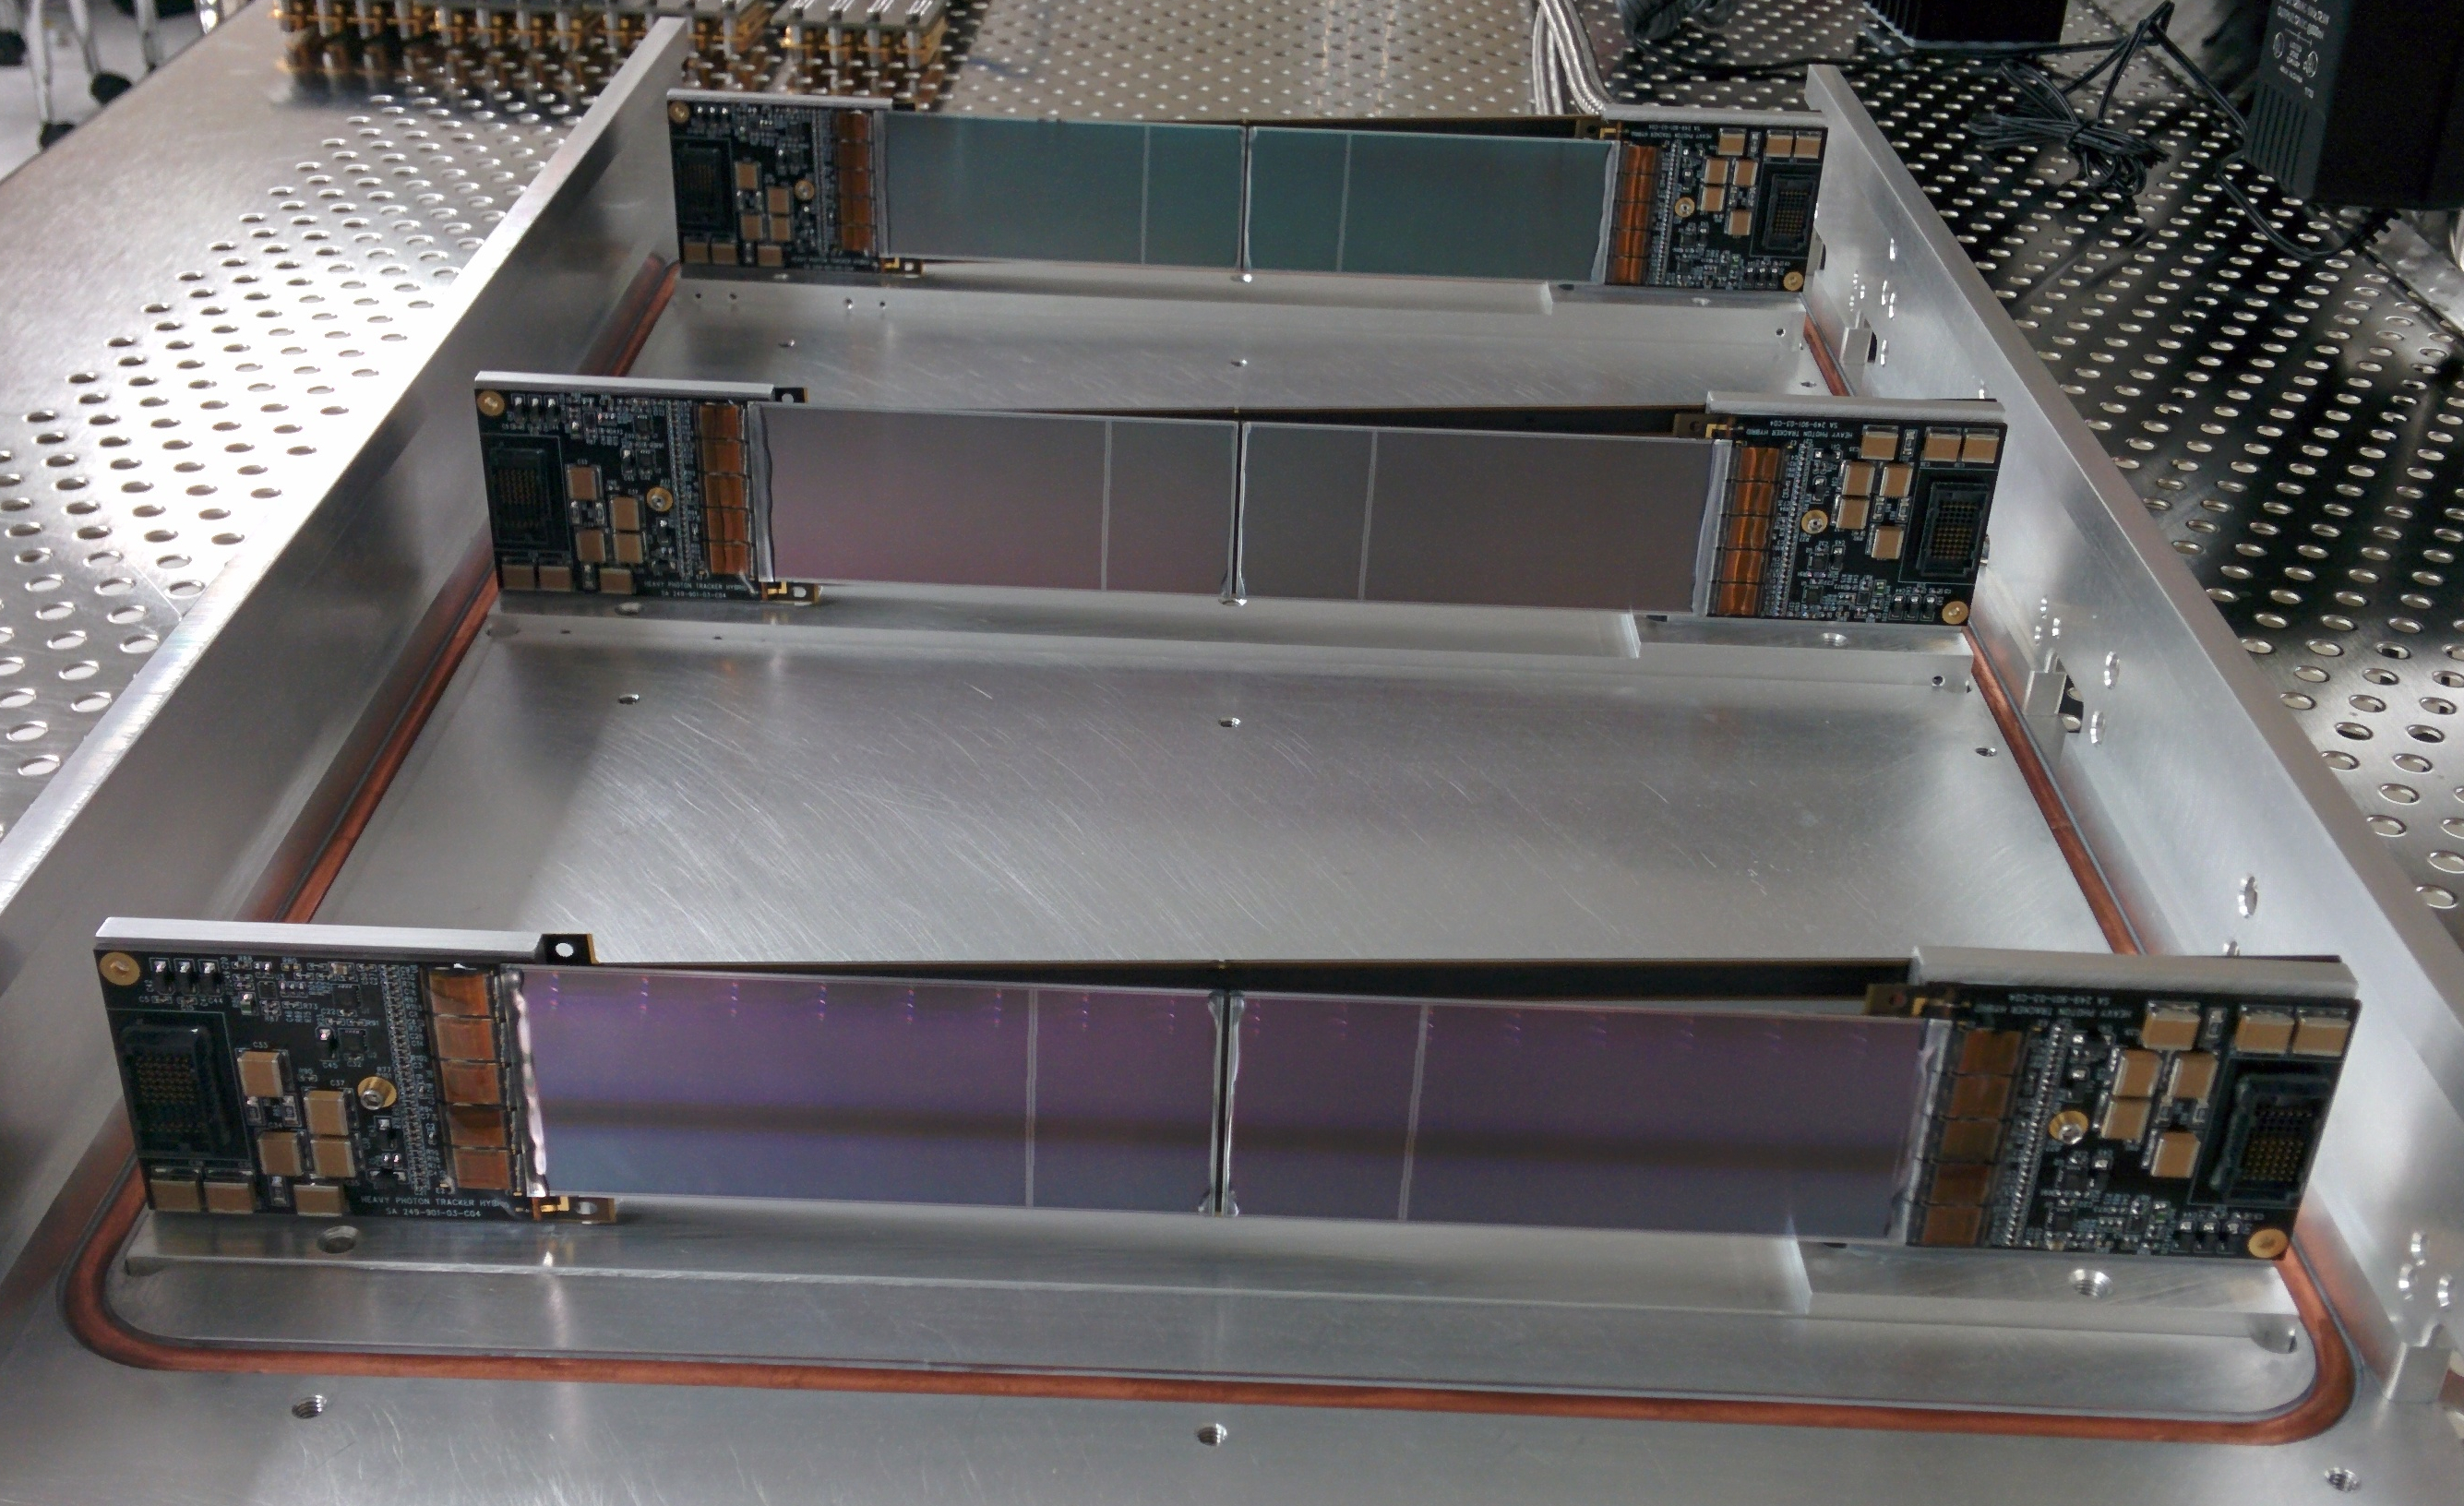
\includegraphics[width=0.9\textwidth]{images/l46_half_module.jpg}
    \caption{A layer 4-6 half-module used by the SVT. }
    \label{fig:l46_hm}
\end{figure}


\subsection{Mechanical Support, Cooling and Services}

...


\section{Electromagnetic Calorimeter}

The HPS Ecal is used as the primary trigger for the experiment as well as to
identify electrons.  It consist of two halves of lead-tungstate 
PbW0$_4$ crystals with each half mounted on an aluminum frame $\sim 137$ cm 
from the upstream edge of the analyzing magnet.  Each half is composed of five
layers of crystals with the four most outer layers consisting of 46 crystals and 
\begin{figure}
    \centering
    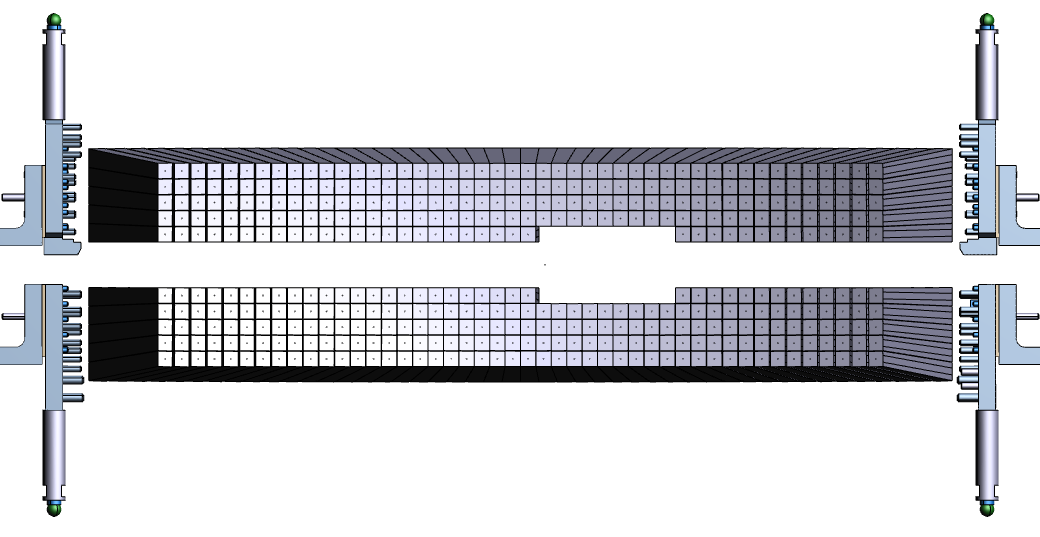
\includegraphics[width=0.8\textwidth]{images/ecal_layout.png}
    \caption{A rendering showing the arrangement of the Ecal crystals.  The Ecal
             is split into upper and lower modules in order to accommodate the 
             ``dead zone''.  The crystals removed from the first layer allow
             a larger opening for the outgoing electron and photon beams.}
    \label{fig:ecal_layout}
\end{figure}
the layer closest to the beam plane consisting of 37. The removal of the 9 
crystals from the inner layer was necessary to allow the outgoing electron and
photon beams to pass through unimpeded.  Each half is enclosed in a temperature
controlled environment held at 1$^{\circ}$ F which encroaches on the Ecal 
vacuum chamber.

Each of the crystals is 16 cm long and trapezoidal in shape with a front face
dimension of $1.3 \times 1.3$ cm$^2$ and a back face dimension of $1.6 \times
1.6$ cm$^2$.  In order to maximize the light yield, the crystals were wrapped
in VM2000 non-metallic reflector film. A Hamamatsu S8664-1010 Avalanche 
Photodiode (APD) with a photosensitive area of $10 \times 10$ mm$^2$ was glued
to the back of each crystal and used to read out the signals collected by the
crystals.  
\begin{figure}
    \centering
    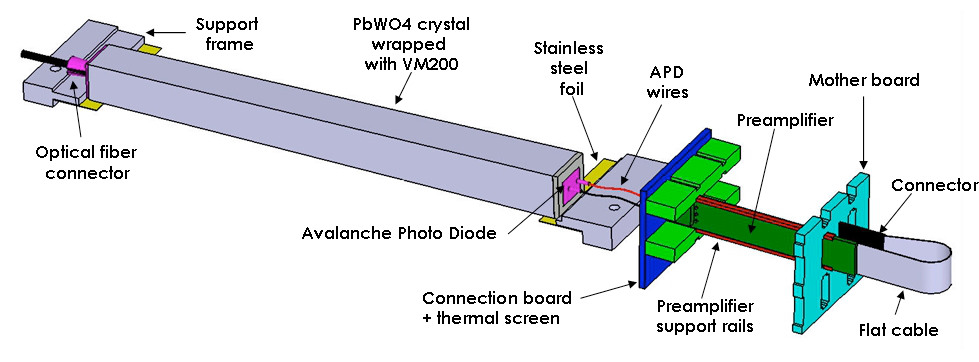
\includegraphics[width=0.8\textwidth]{images/ecal_crystal.png}
    \caption{Rendered view of an HPS Ecal module consisting of a 16 cm PbW$_4$
             crystal, Avalanche Photodiode and preamplifier board.}
    \label{fig:ecal_crystal}
\end{figure}

\section{Trigger and Data Acquisition}

\subsection{Ecal Data Acquisition}

The analog signals that are read out from each of the Ecal crystals by the APDs
are sent a 16-channel JLab FADC250 VXS module (FADC)
(see Figure \ref{fig:ecal_fadc}).  The 221 FADC channels used by each half of 
the Ecal are housed in their own 20 slot VSX crates.
\begin{figure}
    \centering
    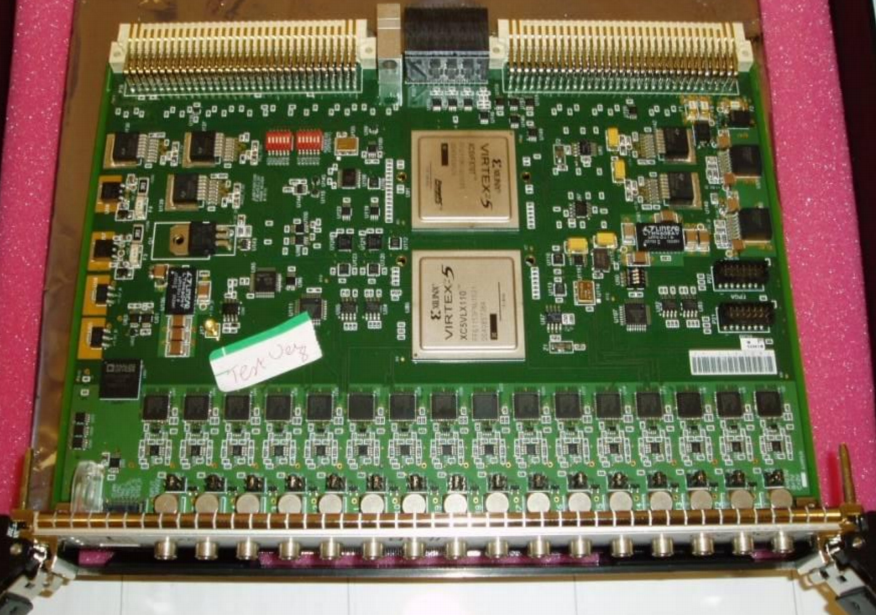
\includegraphics[width=0.7\textwidth]{images/ecal_fadc.png}
    \caption{A 16-channel Jefferson Lab FADC250 VXS module.}
    \label{fig:ecal_fadc}
\end{figure}

The APD signals are sampled and digitized by the FADCs at a rate of 250 MHz
into 8 $\mu$s deep pipelines.  If an FADC signal crosses a pre-defined
threshold, the integrated amplitude of a select number of samples before and
after the threshold crossing, as well as the crossing time are passed to the
Crate Trigger Processor (CTP).

\subsection{Trigger}

The HPS trigger is designed to efficiently select $e^+e^-$ pairs whose energy
depositions, or clusters, in the Ecal are consistent with 
%with either a trident reaction or 
the decay of an $A'$. The trigger logic searches for signals that
are coincident in time and satisfy a specific kinematic selection optimized
to select $A'$ events.

As discussed in the previous section, if a signal from an Ecal crystal is found
to cross some pre-determined threshold, the crossing time and amplitude are 
reported to the CTP. The CTP contains the cluster finding algorithm
which performs the following task: 
\begin{itemize}
    \item The amplitude of hits from every 3x3 array of crystals in the Ecal that
          is within a programmable number of clock cycles is summed. 
    \item If the 3x3 sum exceeds a pre-defined cluster amplitude threshold and
          the sum is greater than any of the neighboring 3x3 windows, then the 
          amplitude (energy), position, time and hit pattern is reported to the Sub-System
          Processor (SSP).
\end{itemize}

The SSP takes the cluster information reported by both halves of the Ecal and
creates all possible pairs of clusters that fall within an 8 ns coincident
window.  Then, in order to further reduce background rates, the following 
selection is applied to the pairs of clusters: 
\begin{itemize}
    \item $E_{min} \le E_{top} + E_{bottom} \le E_{max}$
    \item $| t_{top} - t_{bottom} | \le \Delta t_{max}$
    \item $|E_{top} - E_{bottom} \le \Delta E_{max}$
    \item $E_{low} + R \times  F \le$ Threshold$_{slope}$
    \item $|\tan^{-1}\frac{X_{top}}{Y_{top}} - \tan^{-1}\frac{X_{bottom}}{Y_{bottom}}| \le \theta_{Coplanarity}$
\end{itemize}
Here, $E_{top}$ ($E_{bottom}$), $t_{top}$ ($t_{bottom}$), $x_{top}$ 
($x_{bottom}$) and $y_{top}$ ($y_{bottom}$) are the energy, timestamp and 
position of the cluster in the top (bottom) half of the Ecal and $E_{min}$ 
($E_{max}$) is the minimum (maximum) cluster energy sum. $E_{low}$ is the 
energy of the lowest energy cluster, $R$ is the distance between its 
center and the calorimeter center while $F$ is a constant. As shown on Table
\ref{tab:triggers}, several of these 
parameters are programmable.  The values used during the engineering run are 
listed on Table \ref{tab:triggers}. If a pair of clusters
satisfies these criteria, a trigger signal is generated by the Trigger Supervisor
and sent to all subsystems. 

During the engineering run, several triggers were run simultaneously.  The main
trigger used to select $A'$ type events is the Pair-1 trigger.  The Pair-0 
trigger is a much looser version of the Pair-1 trigger and was tuned to select 
Moller scattering events.  The Single-1 trigger was tuned to select electrons
that Coulomb scatter in the target i.e. full energy electrons (FEE) into the 
acceptance of the Ecal.  These events are used to study both the momentum 
resolution of the tracker and the energy resolution of the Ecal.  Finally, 
there was a cosmic trigger and a pulser trigger used to trigger on cosmic ray
muons and randoms respectively.  A summary of all of the settings is given
on Table \ref{tab:triggers}

\begin{table}
    \centering
    \begin{tabular}{lcccc}
        \toprule
        \textbf{Parameter} & \textbf{Single-0} & \textbf{Single-1} & \textbf{Pair-0} & \textbf{Pair-1} \\
        \midrule
        \midrule
        $E_{min}$ (GeV)      & 0.060 & 0.400 & 0.054 & 0.054 \\
        $E_{high}$ (GeV)     & 2.500 & 1.100 & 1.100 & 0.630 \\
        $N_{threshold}$      & 3     & 3     & 1     & 1     \\
        $E_{sum low}$ (GeV)  &       &       & 0.120 & 0.180 \\
        $E_{sum high}$ (GeV) &       &       & 2.000 & 0.860 \\
        $E_{differenec}$ (GeV) &       &       & 1.000 & 0.540 \\
        $F (GeV)$ & & & 0.0055 \\
        $\theta_{coplanirity}$ & & & 30$^\circ$ \\
        $t_{coplanirity} (ns)$ & & 16 & 12 \\
        Prescale & $2^{13}$ & $2^{11}$ & $2^{10}$ & $2^{0}$ \\
        Rate (50 nA) & 0.4 Hz & 1.3 kHz & 0.7 kHz & 16.6 kHz \\
        \bottomrule
    \end{tabular}
    \caption{The trigger setting for all trigger types used during the 
             engineering run.}
    \label{tab:triggers}
\end{table}



%\subsection{Ecal DAQ}

%\subsection{SVT DAQ}
% Need to discuss the hybrid design for both layers 1-3 and 4-6.
% 1) Need to mention why different wiring was used for the different parts of 
% the SVT.

%After a trigger is received, the differential current signals 
%from each of the APV25's are transferred to a total of 10 Front End Boards (FEB)
%to undergo digitization and further processing. (Add figure?) As discussed in 
%section (), the signals from layers 1-3 are transferred to the FEB's via 
%Teflon-coated twisted pair wires while those emerging from
%layers 4-6 use twisted pair magnet wire.  The use of twisted pairs reduces
%crosstalk between the lines as well as electromagnetic interference.

%At the FEB's, the differential current signals are first converted to a voltage
%by a pre-amplifier circuit to match the dynamic range 
%of the AD9252 14-bit analog to digital converter (ADC). The ADC samples the 
%signal at 41.667 MHz and digitizes it to a value between 0 and 16384.  The 
%digitized signals are then transferred to Xilinx Artix-7 field programmable
%gate arrays (FPGA).  The signals are sent upstream by multi-gigabit transceivers.

%Those signals which pass the threshold requirement are transferred through 
%mini SAS wires to a board on the vacuum  where they undergo optical conversion.
%The optical signal is then transferred over ~10 m fibers to the ATCA crate.


%\subsection{Ecal DAQ}

 % Maybe show an example of how the signal looks emerging from the APV?




%%%%%%%%%%%%%%%%
%   Analysis   %
%%%%%%%%%%%%%%%%
%\chapter{Resonance Search and Results}

After all trident selections applied, the final event sample yield the $e+e-$




%%%%%%%%%%%%%%%%%%%%
%   Bibliography   %
%%%%%%%%%%%%%%%%%%%%
\bibliographystyle{plain}
\bibliography{chapters/bibliography}


%\chapter{HPS Performance Studies}

%\section{Performance of the Silicon Vertex Tracker}
%\subsection{Cluster and Hit Reconstruction}
%\subsection{Tracking Efficiency Using Tag and Probe}
%\subsection{Mass and Vertexing Resolutions}

%\section{Performance of the Electromagnetic Calorimeter}

%\section{Trigger Performance}

%\chapter{Resonance Search and Results}
%\section{Trident Selection}
%\subsection{Selection using Boosted Descision Tree/Random Forest}
%\subsection{Selection using Neural Network}
%\section{Mass Binning}
%\section{Signal and Background Model}
%\section{Systematics}
%\section{Limit Setting}

\end{document}

